\documentclass[a4paper, fleqn]{article}
\usepackage[utf8]{inputenc}
\usepackage{amsmath}
\usepackage{amssymb}
\usepackage{caption}
\usepackage{mathtools}
\usepackage{amsfonts}
\usepackage{lastpage}
\usepackage{tikz}
\usepackage{float}
\usepackage{textcomp}
\usepackage{kbordermatrix}
\usetikzlibrary{patterns}
\usepackage{pdfpages}
\usepackage{gauss}
\usepackage{fancyvrb}
\usepackage[table]{colortbl}
\usepackage{fancyhdr}
\usepackage{graphicx}
\usepackage[margin=2.5 cm]{geometry}

\setlength\parindent{0pt}
\setlength\mathindent{75pt}

\definecolor{listinggray}{gray}{0.9}
\usepackage{listings}
\lstset{
	language=,
	literate=
		{æ}{{\ae}}1
		{ø}{{\o}}1
		{å}{{\aa}}1
		{Æ}{{\AE}}1
		{Ø}{{\O}}1
		{Å}{{\AA}}1,
	backgroundcolor=\color{listinggray},
	tabsize=3,
	rulecolor=,
	basicstyle=\scriptsize,
	upquote=true,
	aboveskip={0.2\baselineskip},
	columns=fixed,
	showstringspaces=false,
	extendedchars=true,
	breaklines=true,
	prebreak =\raisebox{0ex}[0ex][0ex]{\ensuremath{\hookleftarrow}},
	frame=single,
	showtabs=false,
	showspaces=false,
	showlines=true,
	showstringspaces=false,
	identifierstyle=\ttfamily,
	keywordstyle=\color[rgb]{0,0,1},
	commentstyle=\color[rgb]{0.133,0.545,0.133},
	stringstyle=\color[rgb]{0.627,0.126,0.941},
  moredelim=**[is][\color{blue}]{@}{@},
}

\lstdefinestyle{base}{
  emptylines=1,
  breaklines=true,
  basicstyle=\ttfamily\color{black},
}

\pagestyle{fancy}
\def\checkmark{\tikz\fill[scale=0.4](0,.35) -- (.25,0) -- (1,.7) -- (.25,.15) -- cycle;}
\newcommand*\circled[1]{\tikz[baseline=(char.base)]{
            \node[shape=circle,draw,inner sep=2pt] (char) {#1};}}
\newcommand*\squared[1]{%
  \tikz[baseline=(R.base)]\node[draw,rectangle,inner sep=0.5pt](R) {#1};\!}
\newcommand{\comment}[1]{%
  \text{\phantom{(#1)}} \tag{#1}}
\def\el{[\![}
\def\er{]\!]}
\def\dpip{|\!|}
\def\MeanN{\frac{1}{N}\sum^N_{n=1}}
\cfoot{Page \thepage\ of \pageref{LastPage}}
\DeclareGraphicsExtensions{.pdf,.png,.jpg}

\author{Nikolaj Dybdahl Rathcke (Student ID: 74763954)}
\title{Combinatorics \\ Assignment 2}
\lhead{Combinatorics}
\rhead{Assignment 2}

\begin{document}
\maketitle

\section*{Question 1}
\subsection*{Part (a)}
Remember that a transversal matroid is a bipartite graph. Our ground set is the
collection of all elements in the first vertex set $V_1$, and our independent sets,
$\mathcal{I}$, is the collection subsets from $V_1$ that is a matching to the elements in
$V_2$. \\
Construct the bipartite graph, so that all $n$ elements from $V_1$ are connected to the
$r$ elements $V_2$ (a complete graph), then any set with $\leq r$ elements are
independent. Any set with more than $r$ elements will be dependent as there are too many to do a matching. \\
So the uniform matroid $U_{r,n}$ is transversal as long as $r\leq n$.

\subsection*{Part (b)}
We can show this with the counterexample in Figure \ref{fig2}:
\begin{figure}[H]
  \centering
  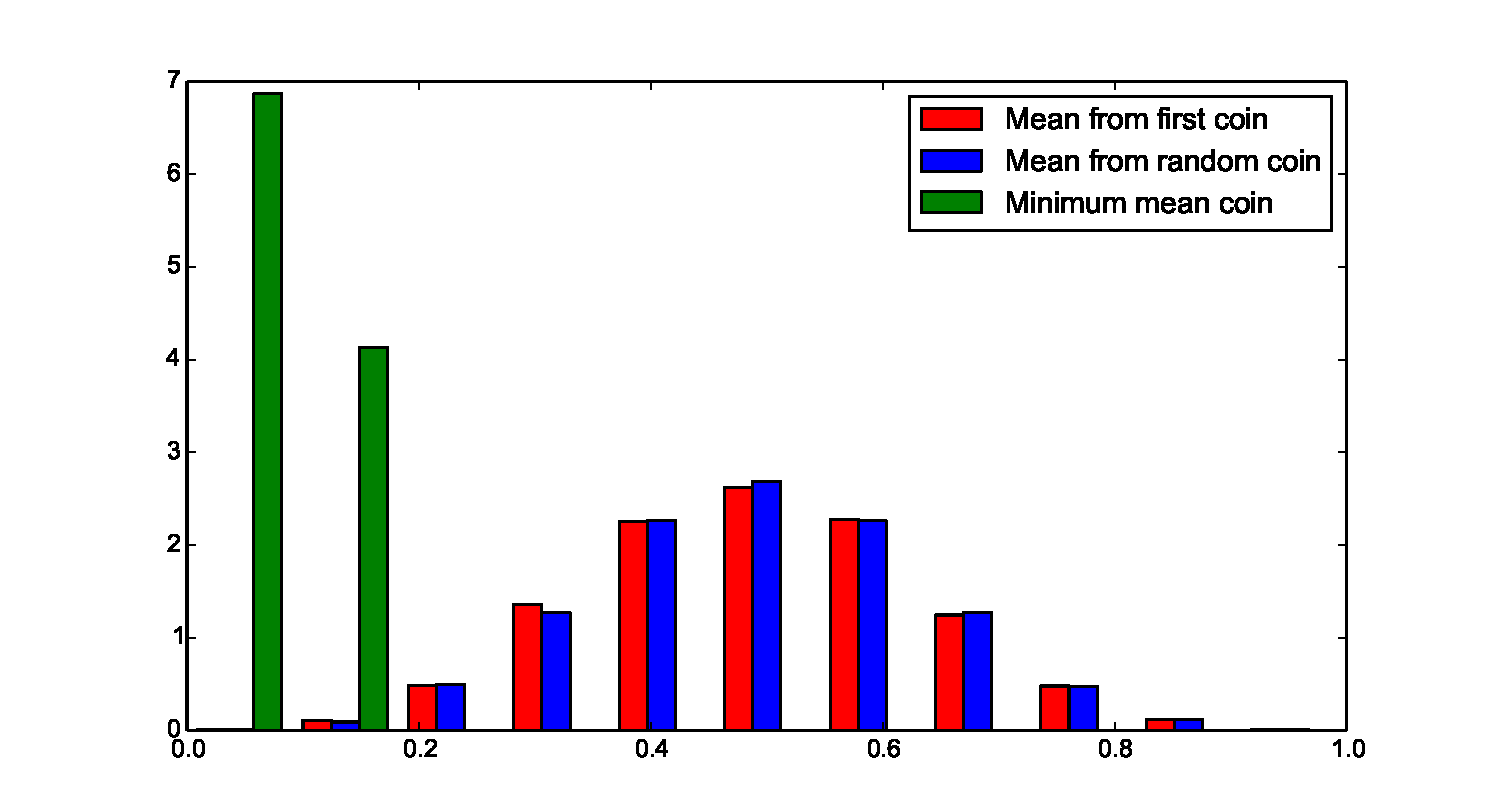
\includegraphics{fig2}
  \caption{A transversal matroid which is not paving.}
  \label{fig2}
\end{figure}
The set $\{a,b\}$ is a circuit of size $2$, but both $\{a,c,d\}$ and $\{b,c,d\}$ are
independent sets (and bases) of size $3$, meaning the matroid has rank $3$.

\subsection*{Part (c)}
Again, we use a counterexample found in Figure \ref{fig3}, which is the cycle graph $C_3$
with parallel edges:
\begin{figure}[H]
  \centering
  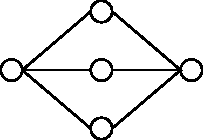
\includegraphics{fig3}
  \caption{A paving matroid which is not transversal.}
  \label{fig3}
\end{figure}
It is paving as it has rank $2$ and minimal circuit size $2$. However it is not
transversal.

\section*{Question 3}
To do this, we need to show that (a) implies (b), that (b) implies (c) and that (c) implies (a).\\
(a) $\Rightarrow$ (b): If $e$ is a loop, then any subset containing $e$ must be dependent and therefore cannot be a basis. \\
(b) $\Rightarrow$ (c): If $e$ is in no bases, then by $(I2)$, it cannot be in any independent sets, as all independent sets in $\mathcal{I}$ are subsets of the bases. \\
(c) $\Rightarrow$ (a): If $e$ is in no independent sets, then it must be a loop, as otherwise the set $\{e\}$ would be an independent set.

\section*{Question 4}
We have that $C$ is a circuit, so $B=C-\{e\}$ must be independent and actually must be a
basis. To see that $C$ must be a unique circuit in $B\cup \{e\}$, say we have another
circuit distinct from $C$ called $C'$, which is contained in $B\cup \{e\}$. Then we must
have that $e\in C\cap C'$ (as otherwise, the circuit is a subset of the basis $B$). By
(\textbf{C3}), we then have that there exists a circuit $C''\subseteq (C\cup C')-\{e\}$,
implying that $C''=B$, which is a contradiction, so $C$ must be unique.

\section*{Question 5}
Not completed.

\section*{Question 6}
The uniform matrix $U_{m,n}$ is graphic for any $n$, where $m$ is an element of the set $\{0,1,n-1, n\}$. The graphs are:
\begin{itemize}
  \item The uniform matroid $U_{0,n}$ is the graphic matroid of the graph with $n$ self-loops.
  \item $U_{1,n}$ is the graphic matroid of the graph where any two vertices that are connected have parallel edges.
  \item $U_{n-1, n}$ is the graphic matroid of the cycle graph $C_{n+1}$ (so it has $n$ edges). If we include all edges, we have a cycle, otherwise we do not.
  \item $U_{n,n}$ is the graphic matroid of any forest with $n$ edges as a tree does not contain a cycle.
\end{itemize}
To realize these are the only ones, assume $U_{m,n}$ is graphical for an $m$ such that $1<m<n-1$. For an independent set $I$ of size $m$, since $m<n-1$, we must have at least $2$ edges that would form a cycle if we added it to $I$. This means that either of the two edges connect two vertices that are already "covered" by the edges in $I$. Therefore, there must exist a subset (or circuit) of size $k\leq \lceil m/2\rceil +1$ that also contains a cycle. Since $k \leq m$ for any $m$, where $1<m<n-1$, that means we have a circuit that has size less than $m+1$, which is a contradiction to the definition of a uniform matroid.

\section*{Question 7}
Not completed.

\section*{Question 8}
We solve this using Prim's algorithm. We start by picking a vertex, say $a$, and then pick the edge with the lowest weight. We keep picking an edge with minimum weight that is adjacent to the tree we are creating, and that includes a vertex that is not currently in the tree. The algorithm runs as follows (use Figure \ref{fig1} for reference:
\begin{enumerate}
  \item Both edges adjacent to $a$ have weight $6$, so it does not matter what we pick. So we pick $(a,b)$.
  \item The edge $(b,e)$ has the lowest weight, so we pick that one.
  \item The edge $(e,f)$ now has the lowest weight, so we pick that one.
  \item We can either pick $(e,g)$ or $(f,g)$ as they both have weight $3$. In this case we pick $(e,g)$.
  \item The edge with lowest weight which includes a vertex not currently in the tree is $(e,c)$.
  \item Finally, we pick the edge $(c,d)$ and we have a minimum spanning tree.
\end{enumerate}
This minimum spanning tree is not unique as we could have picked $(a,g)$ instead of $(a,b)$ as well as $(f,g)$ instead of $(e,g)$.
\begin{figure}[H]
  \centering
  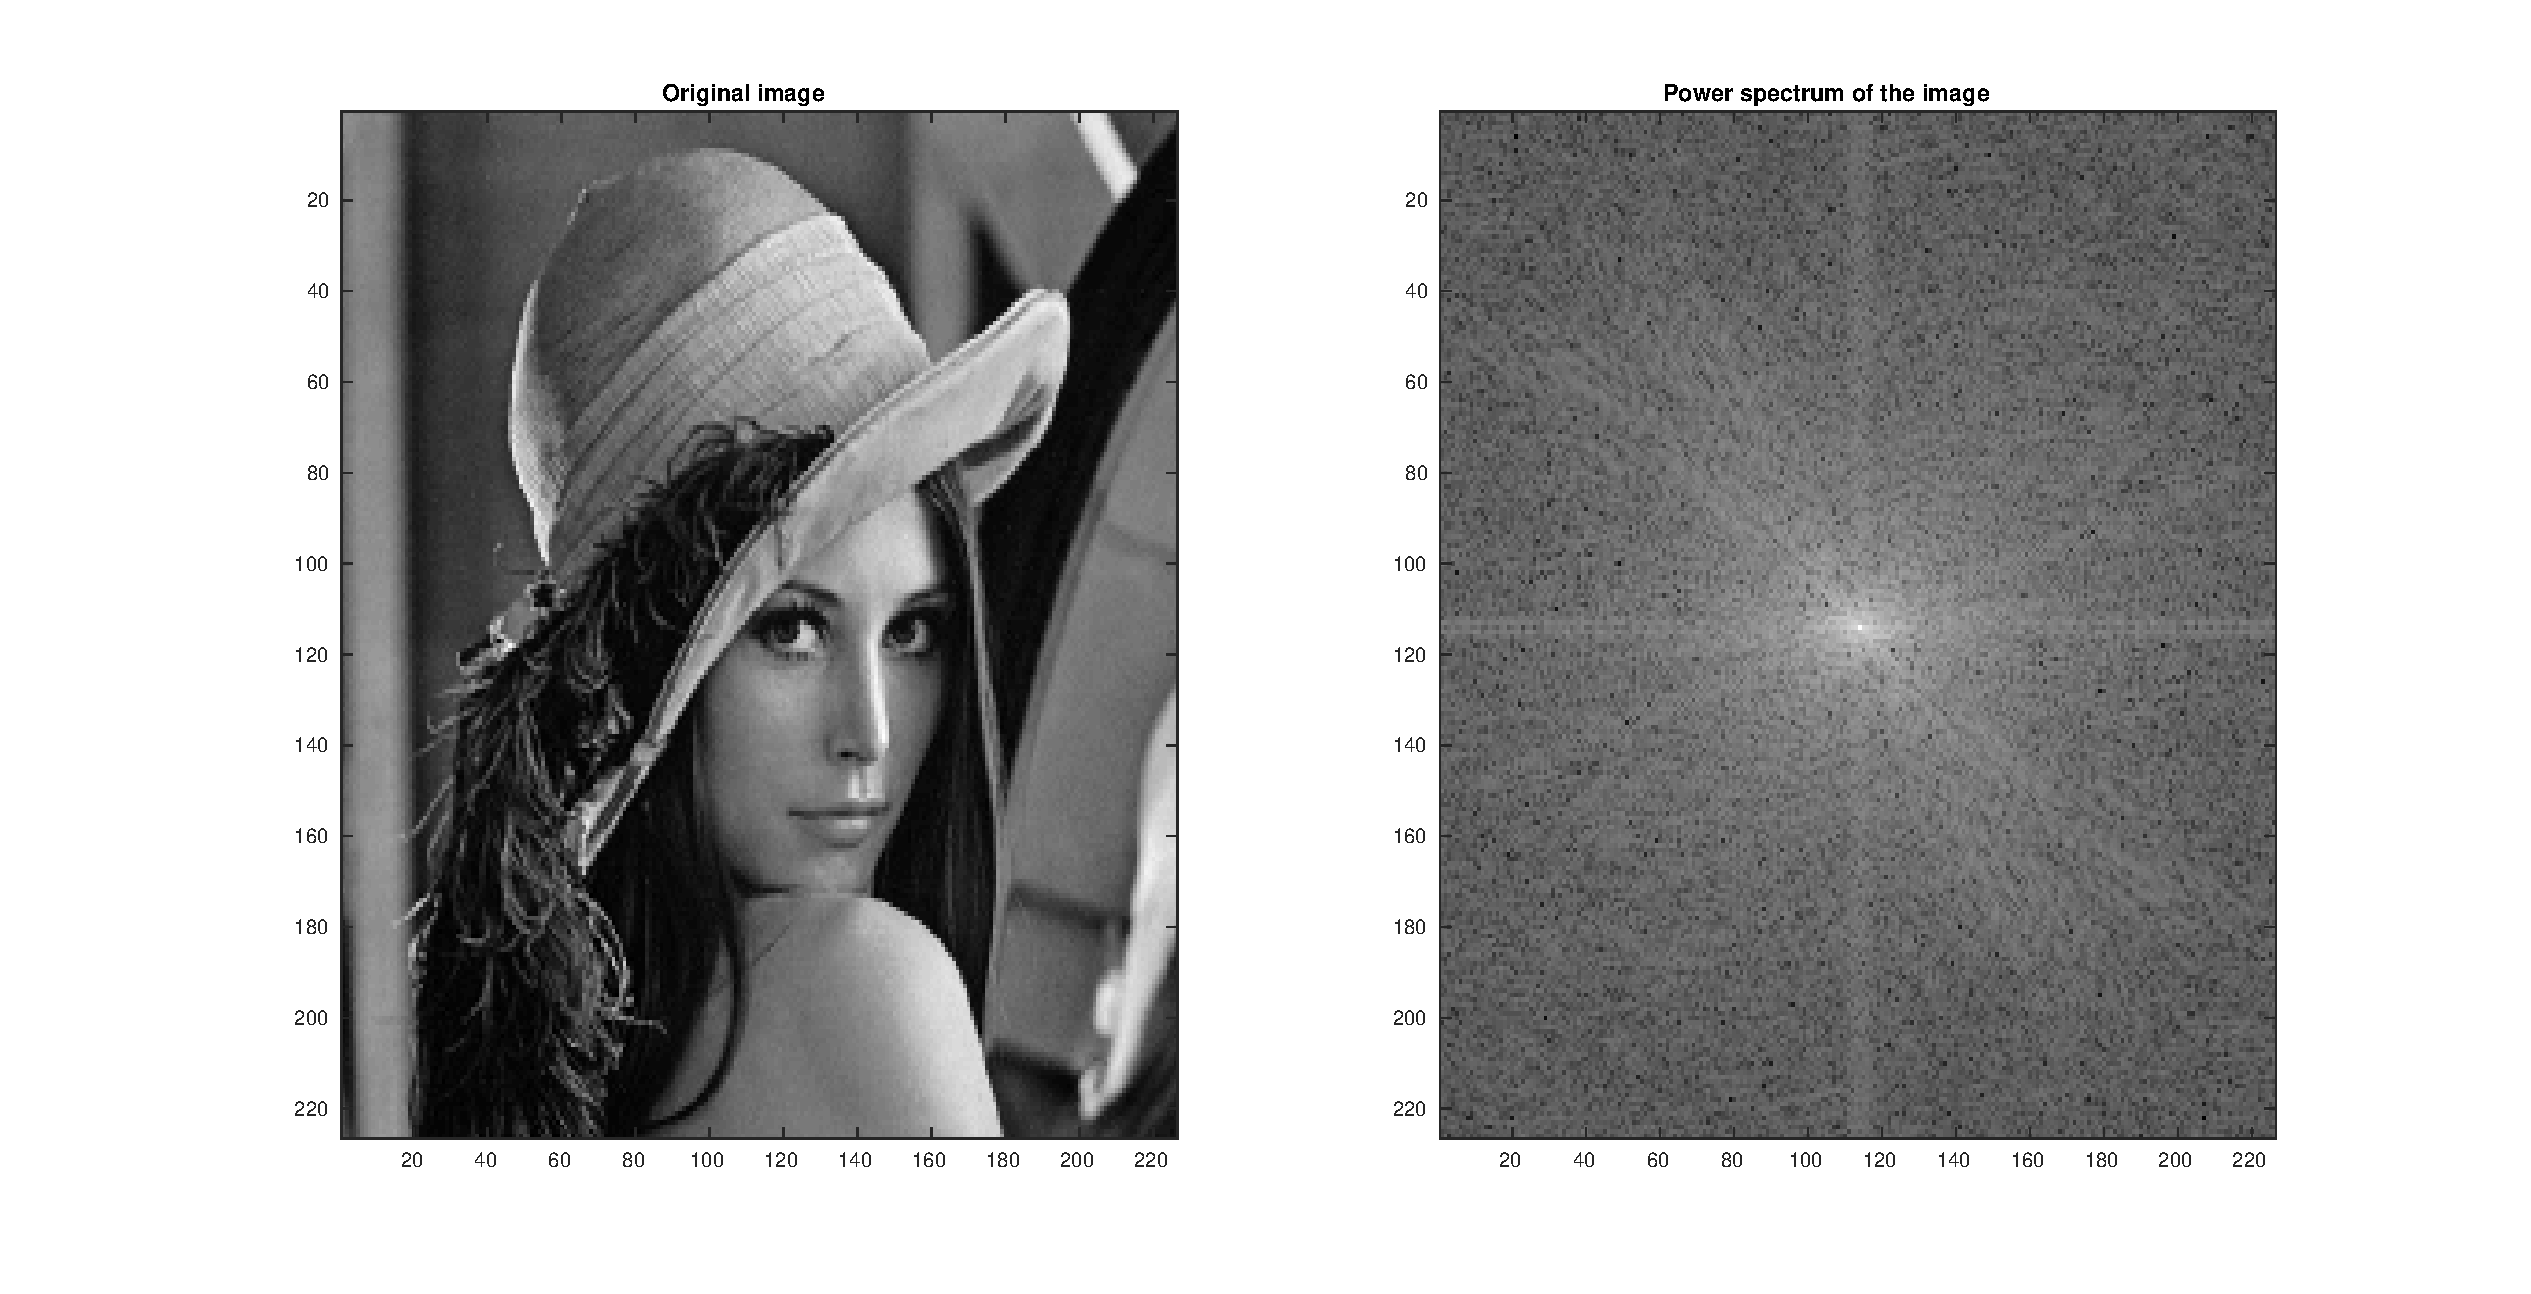
\includegraphics[scale=0.6]{fig1}
  \caption{A minimum spanning tree produced by Prim's Algorithm}
  \label{fig1}
\end{figure}

\section*{Question 9}
Obviously, there must exist a basis with maximal weight as we have a finite number of bases. Let $B_1$ be such a basis. For contradiction, assume that there is another basis $B_2\neq B_1$ with weight $w(B_2)=w(B_1)$. We now pick an element $x\in B_1\Delta B_2$ (the symmetric difference) with \textit{minimum} weight. This element must exist as it is a one-to-one function and $B_1\neq B_2$.  \\
Say that $x\in B_2-B_1$ (without loss of generality), then by (\textbf{B2}), there is an element $y\in B_1-B_2$, so that $B_3=(B_2-\{x\})\cup\{y\}$ is a basis. Since $w(x)<w(y)$, that means $w(B_3)\geq w(B_2)=w(B_1)$, which is a contradiction to the assumption that $B_1$ had maximal weight.

\section*{Question 11}
Not necessarily. Obviously, there might be a matroid whose circuits contain $K$, but this
is not guaranteed. Consider the ground set $E=\{1,2,3,4\}$ with the clutter:
\begin{align*}
  K=\{\{1,2\},\{1,3\},\{2,3,4\}\}
\end{align*}
This is a clutter as no set in the collection is a proper subset of another. If we have a
matroid $M$ where $K\subseteq \mathcal{C}(M)$. \\
Assume that $\mathcal{C}(M)$ must contain all the sets of $K$. If we let $C_1=\{1,2\}$ and
$C_2=\{1,3\}$, then (\textbf{C3}) tells us that that if there is an $e\in C_1\cap C_2$,
then there is another circuit $C_3\subseteq (C_1\cup C_2)-\{e\}$. This means there must be
a circuit $C_3\subseteq \{2,3\}$, but since the set $\{2,3,4\}$ is already in
$\mathcal{C}(M)$, that means $C_3$ must be an independent set in $M$, so $\mathcal{C}(M)$
cannot contain all sets from $K$.





\end{document}
